\documentclass[12pt]{beamer}
\usepackage{../Estilos/BeamerMAF}
\usepackage{../Estilos/ColoresLatex}
%Sección para el tema de beamer, con el theme, usercolortheme y sección de footers
\usetheme{Frankfurt}
\usecolortheme{beaver}
%\useoutertheme{default}
\setbeamercovered{invisible}
% or whatever (possibly just delete it)
\setbeamertemplate{section in toc}[sections numbered]
\setbeamertemplate{subsection in toc}[subsections numbered]
\setbeamertemplate{subsection in toc}{\leavevmode\leftskip=3.2em\rlap{\hskip-2em\inserttocsectionnumber.\inserttocsubsectionnumber}\inserttocsubsection\par}
% \setbeamercolor{section in toc}{fg=blue}
% \setbeamercolor{subsection in toc}{fg=blue}
% \setbeamercolor{frametitle}{fg=blue}
\setbeamertemplate{caption}[numbered]

\setbeamertemplate{footline}
\beamertemplatenavigationsymbolsempty
\setbeamertemplate{headline}{}


\makeatletter
% \setbeamercolor{section in foot}{bg=gray!30, fg=black!90!orange}
% \setbeamercolor{subsection in foot}{bg=blue!30!yellow, fg=red}
% \setbeamercolor{date in foot}{bg=black, fg=white}
\setbeamertemplate{footline}
{
  \leavevmode%
  \hbox{%
  \begin{beamercolorbox}[wd=.333333\paperwidth,ht=2.25ex,dp=1ex,center]{section in foot}%
    \usebeamerfont{section in foot} \insertsection
  \end{beamercolorbox}%
  \begin{beamercolorbox}[wd=.333333\paperwidth,ht=2.25ex,dp=1ex,center]{subsection in foot}%
    \usebeamerfont{subsection in foot}  \insertsubsection
  \end{beamercolorbox}%
  \begin{beamercolorbox}[wd=.333333\paperwidth,ht=2.25ex,dp=1ex,right]{date in head/foot}%
    \usebeamerfont{date in head/foot} \insertshortdate{} \hspace*{2em}
    \insertframenumber{} / \inserttotalframenumber \hspace*{2ex} 
  \end{beamercolorbox}}%
  \vskip0pt%
}







\setbeamercolor{section in foot}{bg=deepcarmine, fg=white}
\setbeamercolor{subsection in foot}{bg=flame, fg=white}
\setbeamercolor{date in foot}{bg=blue, fg=white}

\makeatletter
\setbeamertemplate{footline}
{
\leavevmode%
\hbox{%
\begin{beamercolorbox}[wd=.333333\paperwidth,ht=2.25ex,dp=1ex,center]{section in foot}%
  \usebeamerfont{section in foot} \insertsection
\end{beamercolorbox}%
\begin{beamercolorbox}[wd=.333333\paperwidth,ht=2.25ex,dp=1ex,center]{subsection in foot}%
  \usebeamerfont{subsection in foot}  \insertsubsection
\end{beamercolorbox}%
\begin{beamercolorbox}[wd=.333333\paperwidth,ht=2.25ex,dp=1ex,right]{date in head/foot}%
  \usebeamerfont{date in head/foot} \insertshortdate{} \hspace*{1.5em}
  \insertframenumber{} / \inserttotalframenumber \hspace*{2ex} 
\end{beamercolorbox}}%
\vskip0pt%
}
\makeatother
\usefonttheme{serif}
\setbeamercolor{frametitle}{bg=lavenderblue}
\resetcounteronoverlays{saveenumi}

\date{}

\title{\large{Tema 5 - Legendre con ejercicios}}
\subtitle{Funciones Especiales }
\author{M. en C. Gustavo Contreras Mayén}

\begin{document}
\maketitle
\fontsize{14}{14}\selectfont
\spanishdecimal{.}

\section*{Contenido}
\frame[allowframebreaks]{\tableofcontents[currentsection, hideallsubsections]}

\section{Aplicaciones}
\frame{\tableofcontents[currentsection, hideothersubsections]}
\subsection{Expansión de una función}

%Referencia Hassani. Mathematical methods for students of physics. Example 26.6.1

\begin{frame}
\frametitle{Enunciado}
\textbf{Ejemplo 1.} Queremos encontrar la expansión de Legendre de una función $f (x)$ definida por:
\pause
\begin{align*}
f (x) = \begin{cases}
V_{0} & \text{ si } 0 < x \leq 1 \\
- V_{0} & \text{ si } -1 \leq x < 0
\end{cases}
\end{align*}
\end{frame}
\begin{frame}
\frametitle{Ocupando expresiones}
Utilizamos las ecuaciones:
\pause
\begin{align*}
f (x) = \nsum_{\ell = 0}^{\infty} a_{\ell} \, P_{\ell} (x)
\end{align*}
y
\pause
\begin{align*}
a_{\ell} = \dfrac{2 \, \ell + 1}{2} \, \scaleint{6ex}_{-1}^{1} f (x) \, P_{\ell} (x) \dd{x}
\end{align*}
\end{frame}    
\begin{frame}
\frametitle{Calculando coeficientes}
\begin{eqnarray*}
\begin{aligned}
&a_{\ell} = \dfrac{2 \ell + 1}{2} \scaleint{6ex}_{-1}^{1} f (x) P_{\ell} (x) \dd{x} = \\[1em] \pause
&= \dfrac{2 \ell + 1}{2} \scaleint{6ex}_{-1}^{0} \underbrace{f (x)}_{=-V_0}  P_{\ell} (x) \dd{x} + \\[0.5em]
&+ \dfrac{2 \ell + 1}{2} \scaleint{6ex}_{0}^{1} \underbrace{f (x)}_{=+V_0}  P_{\ell} (x) \dd{x}
\end{aligned}
\end{eqnarray*}
\end{frame}
\begin{frame}
\frametitle{Calculando coeficientes}
\begin{align*}
= \dfrac{2 \ell + 1}{2} V_{0} \left[ - \scaleint{6ex}_{-1}^{0} P_{\ell} (x) \dd{x} + \scaleint{6ex}_{0}^{1} P_{\ell} (x) \dd{x} \right]
\end{align*}
\end{frame}
\begin{frame}
\frametitle{Haciendo un cambio de variable}
En la primera integral de la última línea, hacemos el cambio de variable $x = -y$, por lo que:
\pause
\begin{eqnarray*}
\begin{aligned}
&\scaleint{6ex}_{-1}^{0} P_{\ell} (x) \dd{x} = \scaleint{6ex}_{+1}^{0} P_{\ell} (-y) (-\dd{y}) =  \\[0.5em] \pause
&= \scaleint{6ex}_{0}^{1} P_{\ell} (-y) \dd{y} = \\[0.5em] \pause
&= (-1)^{\ell} P_{\ell} (x) \dd{x}
\end{aligned}
\end{eqnarray*}
\end{frame}
\begin{frame}
\frametitle{Usando propiedades}
Donde ocupamos una de la propiedad de paridad de los polinomios de Legendre:
\pause
\begin{align*}
P_{\ell} (-u) = (-1)^{\ell} \, P_{\ell} (u)
\end{align*}
\pause
Sustituimos en la expresión para los coeficientes:
\end{frame}
\begin{frame}
\frametitle{Sustituyendo}
\begin{eqnarray*}
\begin{aligned}
&a_{\ell} = \dfrac{2 \ell + 1}{2} \, V_{0} \,  [1 - (-1)^{\ell} ] \scaleint{6ex}_{0}^{1} P_{\ell} (x) \dd{x} = \\[1em] \pause
&= \dfrac{2 \ell + 1}{2} \, V_{0} \begin{cases}
0 & \text{ si } \ell \text{ es par} \\
\displaystyle 2  \, \scaleint{6ex}_{0}^{1} P_{2 k + 1} (x) \dd{x} & \text{ si } \ell 
\end{cases} = \\[0.5em] \pause
&= 2 k + 1 
\end{aligned}
\end{eqnarray*}
\pause
$\ell$ impar es $\ell = 2 k + 1$ con $k = 0, 1, 2, \ldots$.
\end{frame}
\begin{frame}
\frametitle{Evaluando la integral}
Queda por evaluar la integral del polinomio de Legendre de orden impar en el intervalo $(0, 1)$. \pause Para ello, utilizamos la fórmula de Rodrigues:
\pause
\begin{align*}
&\scaleint{6ex}_{0}^{1} P_{2k+1} (x) \dd{x} = \dfrac{1}{2^{2k+1} \; (2k +1)!} \times \\[0.5em]
&\times \scaleint{6ex}_{0}^{1} \dv[2k+1]{x} \left[ (x^{2} - 1)^{2k+1} \right] \dd{x} = 
\end{align*}
\end{frame}
\begin{frame}
\frametitle{Evaluando la integral}
\begin{eqnarray*}
\begin{aligned}
&= \dfrac{1}{2^{2k+1} \; (2k +1)!} \; \dv[2k]{x} \left[ (x^{2} - 1)^{2k+1} \right] \eval_{0}^{1} = \\[1em] \pause
&= \dfrac{1}{2^{2k+1} \; (2k +1)!} \; \left\{ \dv[2k]{x} \left[ (x^{2} - 1)^{2k+1} \right] \eval_{x=1} + \right. = \\[1em] \pause
&- \left. \dv[2k]{x} \left[ (x^{2} - 1)^{2k+1} \right] \eval_{x=0} \right\}
\end{aligned}
\end{eqnarray*}
\end{frame}
\begin{frame}
\frametitle{Revisando los resultados}
El primer término resulta ser cero, \pause porque no hay un número suficiente de diferenciaciones para deshacerse de todos los factores de $(x^{2} - 1)$. 
\\
\bigskip
\pause
Para el segundo término, observamos que $(x^{2} - 1)^{2k + 1}$ es un polinomio en $x$ cuyos derivadas de varios órdenes, serán potencias de $x$.
\end{frame}
\begin{frame}
\frametitle{Revisando los resultados}
Estas potencias devolverán cero en $x = 0$, excepto para el término constante (de potencia cero).
\\
\bigskip
\pause
Por lo tanto, vamos a utilizar la expansión binomial para $(x^{2} - 1)^{2k + 1}$, que es igual a $-(1 - x^{2})^{2k + 1}$:
\end{frame}
\begin{frame}
\frametitle{Usando la expansión binomial}
\begin{eqnarray*}
\begin{aligned}
&\dv[2k]{x} \bigg[ (x^{2} - 1)^{2k+1} \bigg] \eval_{x=0} = \\[0.5em] \pause
&- \dv[2k]{x} \bigg[ \nsum_{j=0}^{2k+1} \dfrac{(2k+1)!}{j! \, (2k + 1 - j)!}  (-x^{2})^{j} \bigg] \eval_{x=0} \\[1em] \pause
&= - \nsum_{j=0}^{2k+1} \dfrac{(2k+1)!}{j! \; (2k + 1 - j)!} \, (-1)^{j} \dv[2k]{x} \left( x^{2j} \right) \eval_{x=0}
\end{aligned}
\end{eqnarray*}
\end{frame}
\begin{frame}
\frametitle{Usando la expansión binomial}
De donde se obtiene un término constante cuando $k = j$:
\setbeamercolor{item projected}{bg=cinnabar,fg=white}
\setbeamertemplate{enumerate items}{%
\usebeamercolor[bg]{item projected}%
\raisebox{1.5pt}{\colorbox{bg}{\color{fg}\footnotesize\insertenumlabel}}%
}
\begin{enumerate}[<+->]
\item Todos los demás términos de la suma se anulan ya sea por tener demasiadas diferenciaciones (cuando $j <k$, terminamos derivando constantes).
\item O por tener muy pocas diferenciaciones (cuando $j> k$, una potencia de $x$ permanece y se evalúa como cero en $x = 0$).
\end{enumerate}
\end{frame}
\begin{frame}
\frametitle{Usando la expansión binomial}
Por tanto:
\pause
\begin{eqnarray*}
\begin{aligned}
&\dv[2k]{x} \left[ (x^{2} - 1)^{2k+1} \right] \eval_{x=0} = \\[0.5em] \pause 
&- \dfrac{(2 k + 1)!}{k! \, (k + 1)!} \, (-1)^{k} \dv[2k]{x} \left( x^{2 k} \right) \eval_{x=0} \\[1em] \pause
&= \dfrac{(2 k + 1)!}{k! \; (k + 1)!} \, (-1)^{k+1} \, (2 \, k)!
\end{aligned}
\end{eqnarray*}
\end{frame}
\begin{frame}
\frametitle{Expresión para el coeficiente}
Entonces el coeficiente $a_{2k+1}$ se escribe como:
\pause
\begin{eqnarray*}
\begin{aligned}
&a_{2k+1} = 2 \, \dfrac{2 \, (2 k + 1) + 1}{2} \, V_{0} \, \scaleint{6ex}_{0}^{1} P_{2k+1} (x) \dd{x} = \\[0.5em] \pause
&= \dfrac{(-1)^{k} \, (4 k + 3) \, (2 k!)}{2^{2 k + 1} \, k! \, (k + 1)!} \, V_{0}
\end{aligned}
\end{eqnarray*}
con $a_{\ell} = 0$ para $\ell$ par. 
\end{frame}
\begin{frame}
\frametitle{Expansión de la función}
La expansión final en series se escribe como:
\pause
\begin{eqnarray*}
\begin{aligned}
&f (x) = \begin{cases}
V_{0} & \text{ si } 0 < x \leq 1 \\
-V_{0} & \text{ si } -1 \leq x < 0
\end{cases} = \\[0.5em] \pause
&= V_{0} \, \nsum_{k=0}^{\infty} \dfrac{(-1)^{k} \,(4 k + 3) \, (2 k!)}{2^{2 k + 1} \, k! \, (k + 1)!} \, P_{2k+1} (x)
\end{aligned}
\end{eqnarray*}
\end{frame}
\begin{frame}
\frametitle{Primeros términos}
Expresando los primeros términos:
\pause
\begin{align*}
f (x) = V_{0} \, \left[ \dfrac{3}{2} P_{1}(x) - \dfrac{7}{4} P_{3}(x) + \dfrac{21}{16} P_{5}(x) - \cdots \right]
\end{align*}
\end{frame}
\begin{frame}[plain]
\begin{figure}
    \centering
    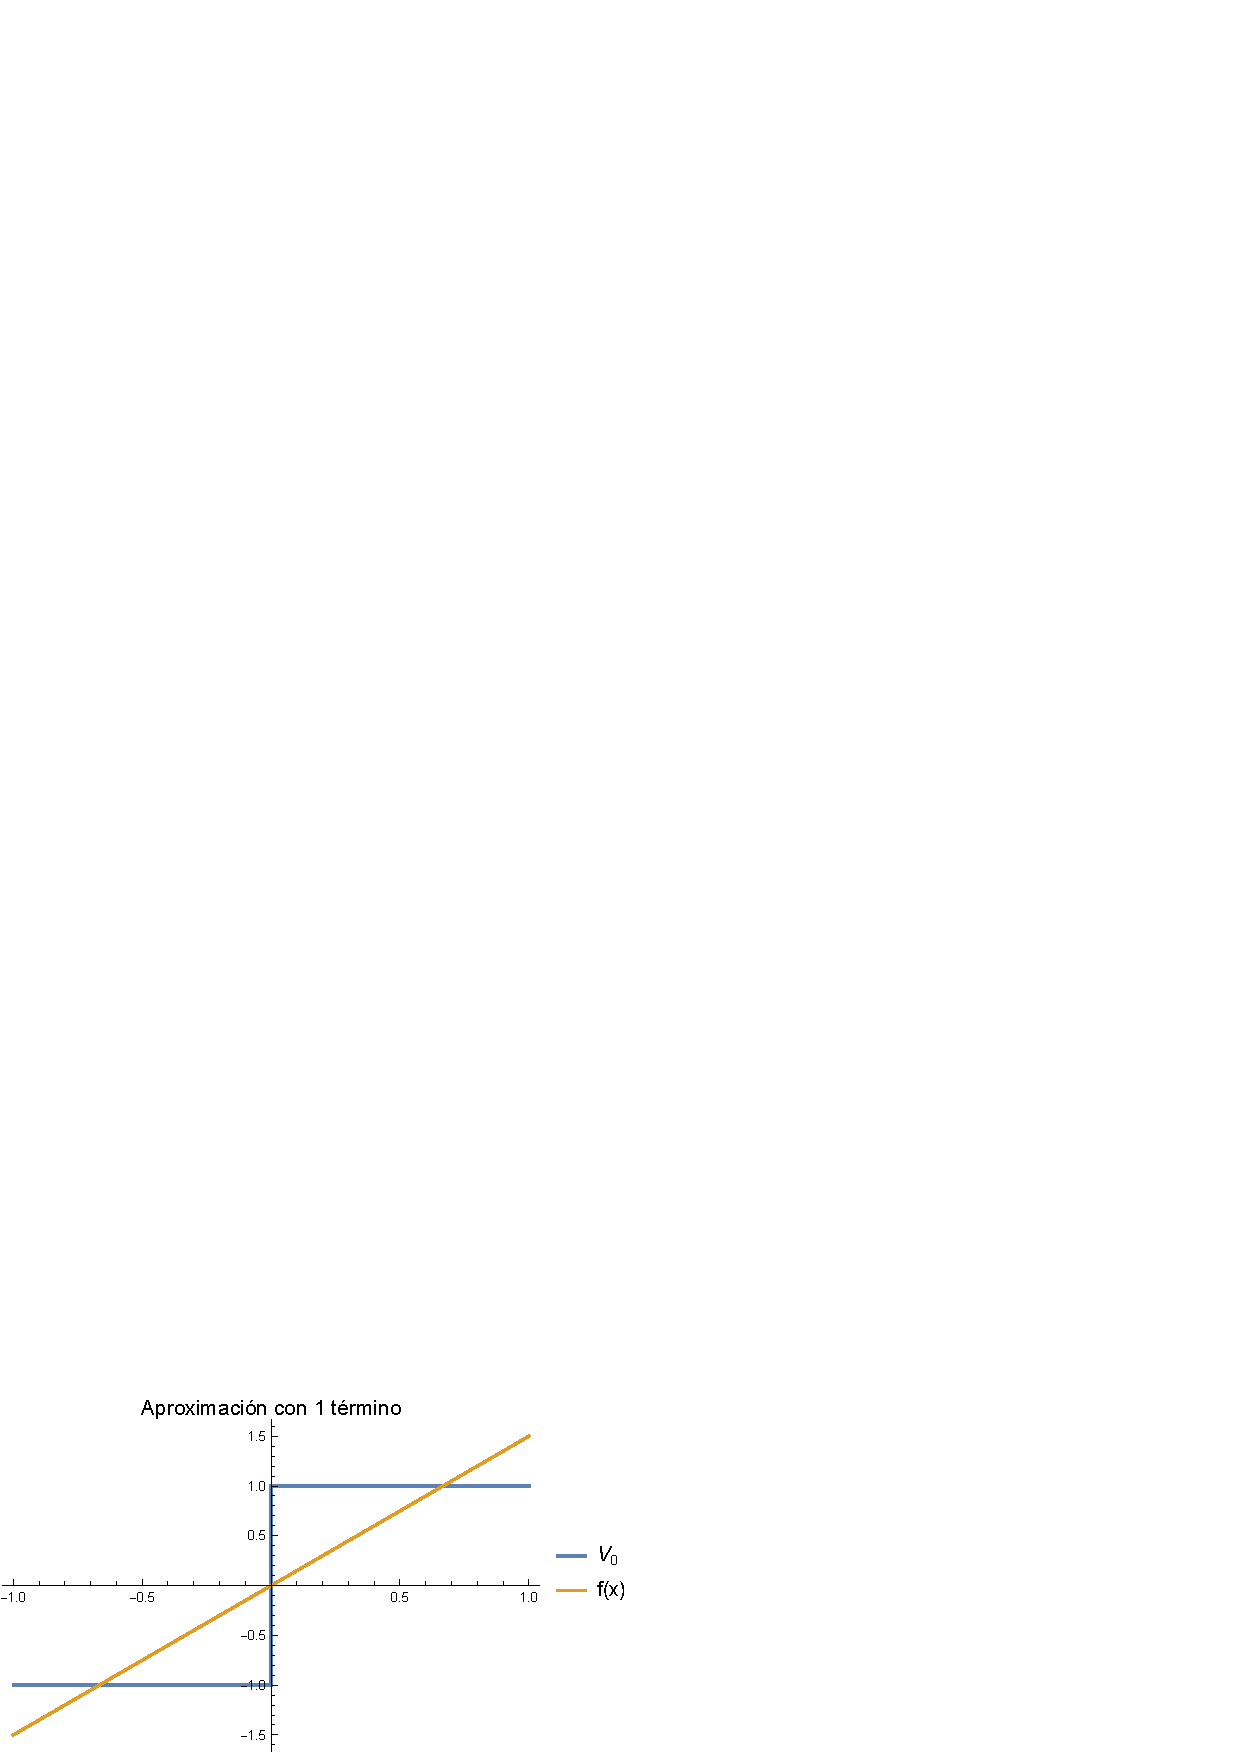
\includegraphics[scale=0.7]{Imagenes/Legendre_Expansion_01.pdf}
\end{figure}
\end{frame}
\begin{frame}[plain]
\begin{figure}
    \centering
    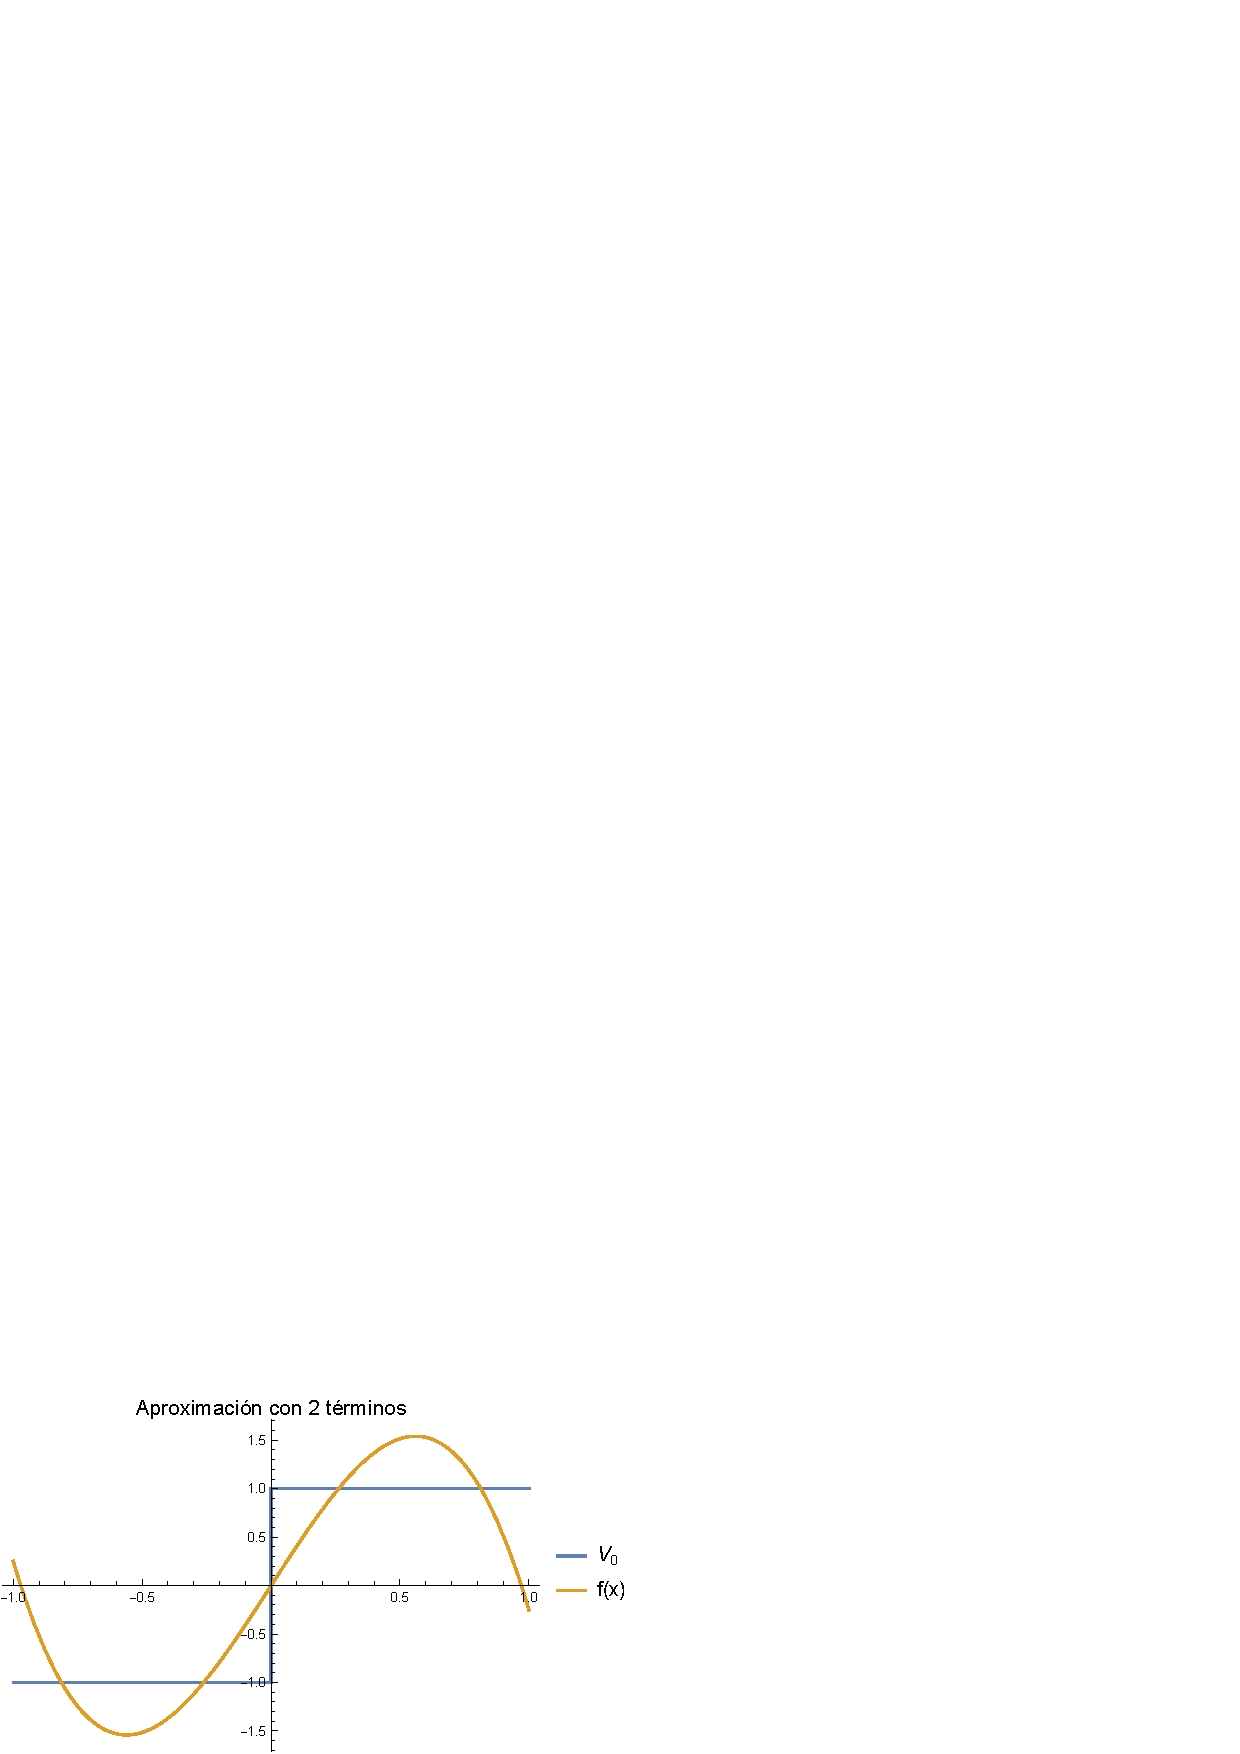
\includegraphics[scale=0.7]{Imagenes/Legendre_Expansion_02.pdf}
\end{figure}
\end{frame}
\begin{frame}[plain]
\begin{figure}
    \centering
    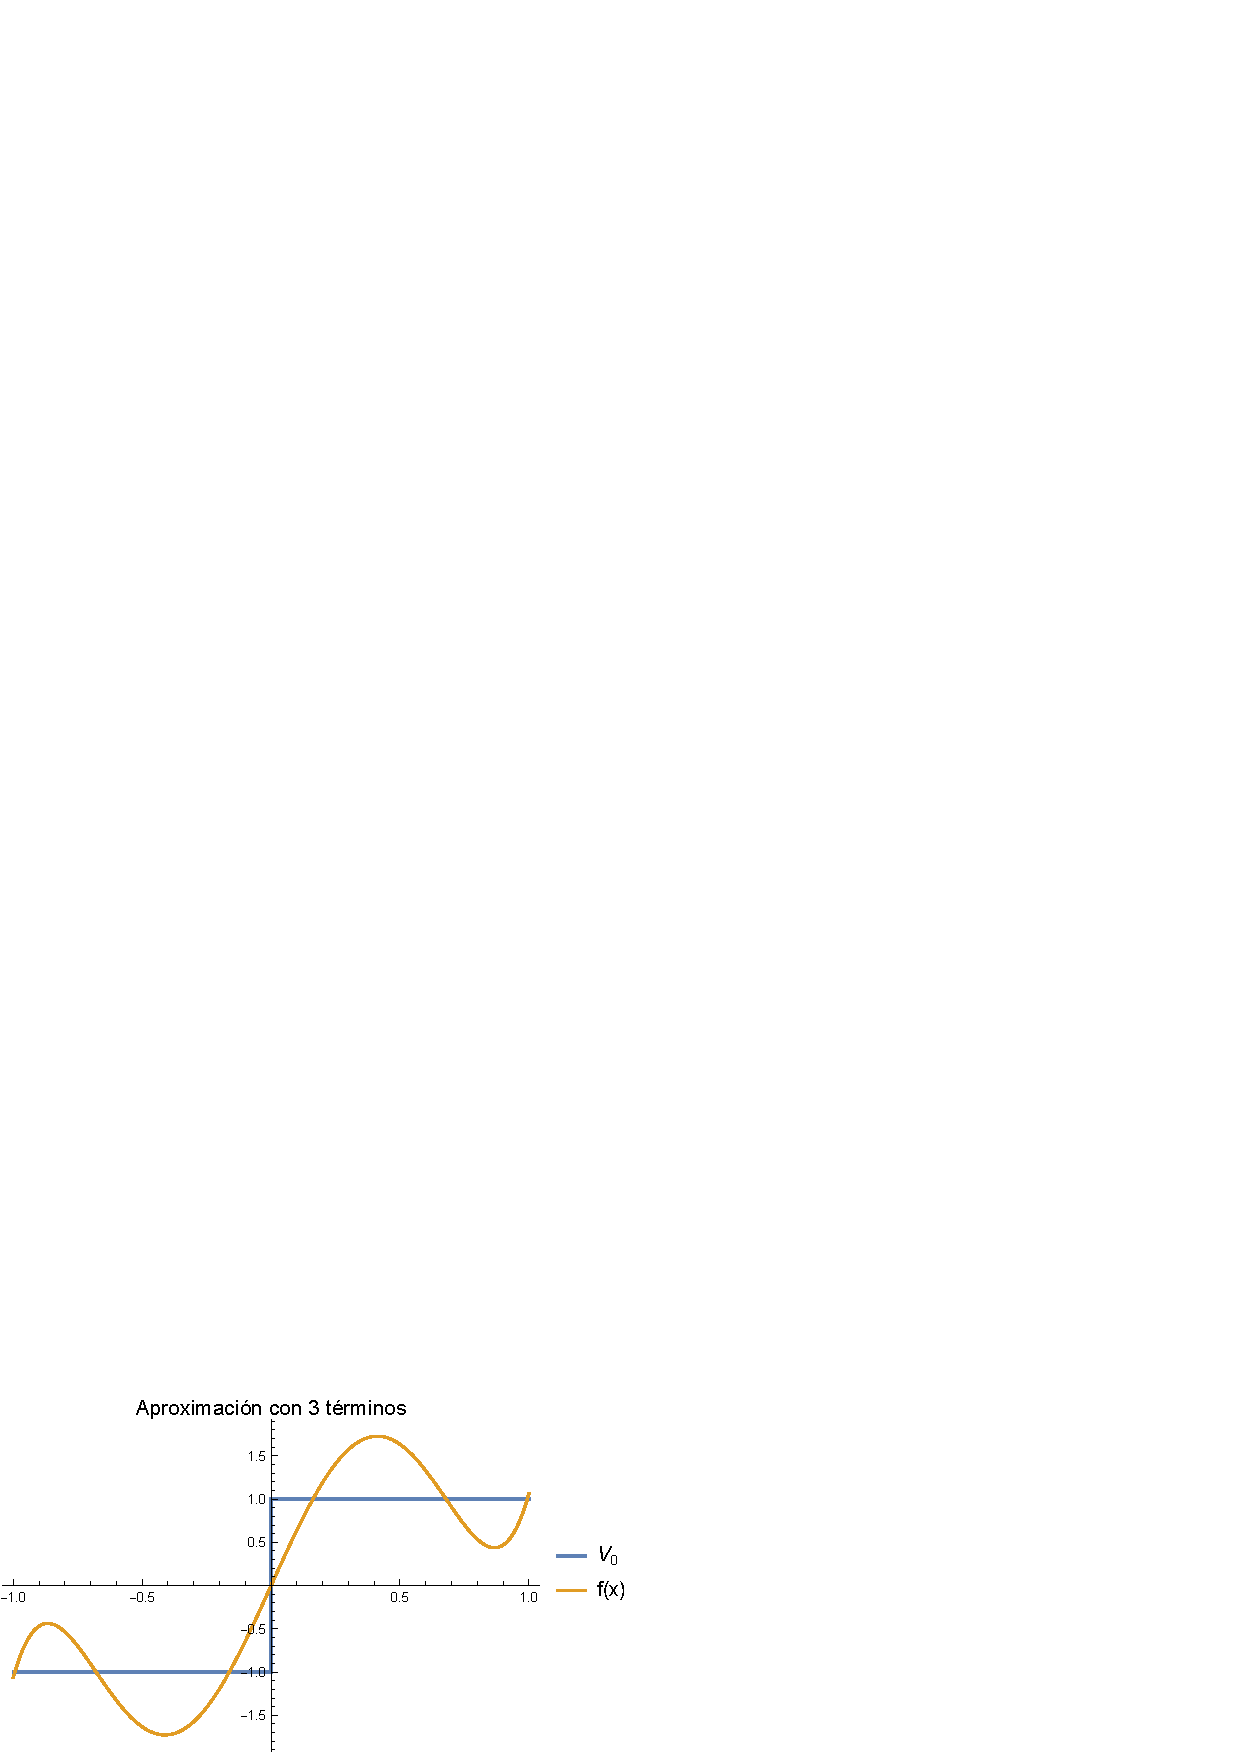
\includegraphics[scale=0.7]{Imagenes/Legendre_Expansion_03.pdf}
\end{figure}
\end{frame}
\begin{frame}[plain]
\begin{figure}
    \centering
    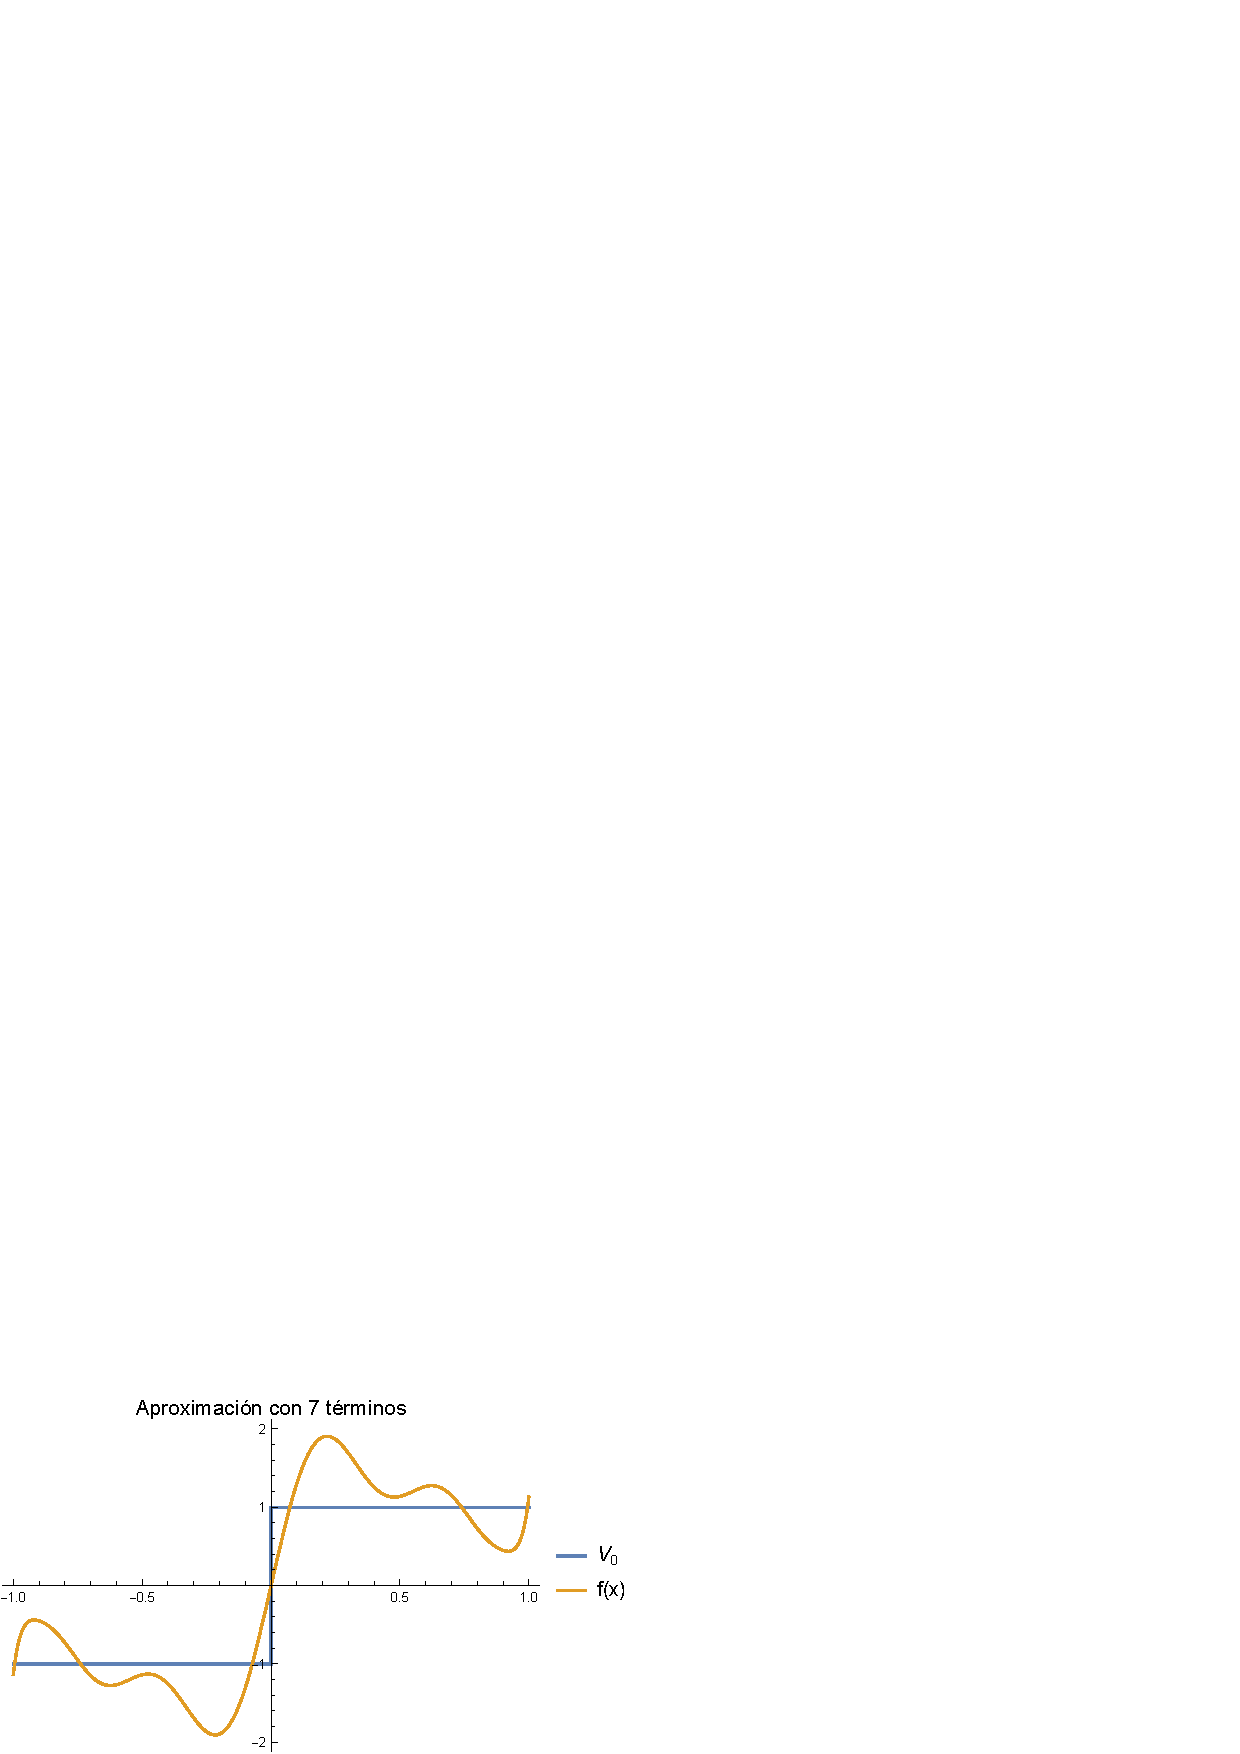
\includegraphics[scale=0.7]{Imagenes/Legendre_Expansion_04.pdf}
\end{figure}
\end{frame}

\section{Cálculo de potenciales eléctricos}
\frame{\tableofcontents[currentsection, hideothersubsections]}
\subsection{Revisando el ejercicio}

\begin{frame}
\frametitle{Enunciado del problema}
Considera un arreglo de cargas en el eje $x$:
\pause
\begin{itemize}[<+->]
\item Una carga $+q$ está en la posición $x = -a$.
\item Una carga $-2 \, q$ está en la posición $x = 0$.
\item Una carga $+q$ está en la posición $x = a$.
\end{itemize}
\end{frame}
\begin{frame}
\frametitle{Geometría del problema}
Haciendo un esquema del problema tenemos que:
\pause
\begin{figure}
    \centering
    \includestandalone[scale=0.9]{Figuras/cuadrupolo_01}
\end{figure}
\pause
Calcula el potencial electrostático de este arreglo, conocido como el \textocolor{cobalt}{cuadruplo lineal eléctrico}.
\end{frame}

\subsection{Solución}

\begin{frame}
\frametitle{Estableciendo el potencial}
Como se revisó en el curso de Electromagnetismo, es posible describir el potencial debido a las tres cargas:
\pause
\begin{align}
V = k \, q \, \left( \dfrac{1}{r_{1}} + \dfrac{1}{r_{2}} \right) - \dfrac{2 \, k \, q}{r}
\label{eq:ecuacion_01}
\end{align}
\end{frame}
\begin{frame}
\frametitle{Estableciendo el potencial}
\begin{figure}
    \centering
    \includestandalone[scale=0.7]{Figuras/cuadrupolo_02}
\end{figure}
\pause
\fontsize{12}{12}\selectfont
donde:
\begin{itemize}[<+->]
\item $r_{1}$ es la distancia de la carga ($0, -a)$ al punto $P$.
\item $r_{2}$ es la distancia de la carga ($0, +a)$ al punto $P$.
\item $r$ es la distancia de la carga en el origen al punto $P$.
\end{itemize}
\end{frame}
\begin{frame}
\frametitle{Solución}
A partir de la ley de los cosenos escribimos $r_{1}$ y $r_{2}$:
\pause
\begin{eqnarray*}
\begin{aligned}
r_{1}^{2} &= r^{2} + a^{2} - 2 \, a \, r \, \cos \theta =  \\[0.5em] \pause 
r_{1} &= r \sqrt{1 + \left( \dfrac{a}{r} \right)^{2} - 2 \left( \dfrac{a}{r} \right) \, \cos \theta}
\end{aligned}
\end{eqnarray*}
\end{frame}
\begin{frame}
\frametitle{Solución}
Para $r_{2}$:
\pause
\begin{eqnarray*}
\begin{aligned}
r_{2}^{2} &= r^{2} + a^{2} + 2 \, a \, r \, \cos \theta =  \\[0.5em] \pause
r_{2} &= r \sqrt{1 + \left( \dfrac{a}{r} \right)^{2} + 2 \left( \dfrac{a}{r} \right) \, \cos \theta}
\end{aligned}
\end{eqnarray*}
\end{frame}
\begin{frame}
\frametitle{Uso de los polinomios de Legendre}
Sabemos que la expresión para el potencial es muy similar a la función generatriz de los polinomios de Legendre.
\\
\bigskip
\pause
Si nos enfocamos solamente en el potencial de las dos cargas en $(0, \pm a)$:
\end{frame}
\begin{frame}
\frametitle{Potencial de las dos cargas}
El potencial debido a esas dos cargas es:
\pause
\begin{align}
\begin{aligned}
V_{\pm a} &= \dfrac{k \, q}{r} \bigg[ \sum_{n=0}^{\infty} \left( \dfrac{a}{r} \right)^{\ell} P_{\ell}(x) + \\[0.5em]
&+ \sum_{n=0}^{\infty} (-1)^{\ell} \left( \dfrac{a}{r} \right)^{\ell} P_{\ell}(x) \bigg]
\end{aligned}
\label{eq:ecuacion_03}
\end{align}
\end{frame}
\begin{frame}
\frametitle{La expresión obtenida}
Vemos que la ec. (\ref{eq:ecuacion_03}) es muy similar a la expresión para el dipolo eléctrico lineal.
\\
\bigskip
\pause
La diferencia es que las dos sumas suman (en lugar de restar); esto ocurre porque las dos cargas en $(0, \pm a)$ son positivas, en lugar de tener signos opuestos como en el caso del dipolo.
\end{frame}
\begin{frame}
\frametitle{La expresión obtenida}
Observemos el término $(-1)^{\ell}$ en la segunda suma: esto surge de la expresión de la ley de cosenos para $r_{2}$, en la que el ángulo entre $r$ y $a$ es $(\ang{180} - \theta)$, de modo que $\cos (\ang{180} - \theta) = - \cos \theta$.
\end{frame}
\begin{frame}
\frametitle{Revisando la expresión}
Si revisamos la ec. (\ref{eq:ecuacion_03}), nos damos cuenta de que las sumas se anula si $n$ es impar, dejándonos solo los términos pares:
%\fontsize{12}{12}\selectfont
\begin{align}
\begin{aligned}
V_{\pm a} &= \dfrac{2 \, k \, q}{r} \bigg[ P_{0} \left( \dfrac{a}{r} \right)^{0} + P_{2} \left( \dfrac{a}{r} \right)^{2} \, P_{4} \left( \dfrac{a}{r} \right)^{4} + \ldots \bigg]
\end{aligned}
\label{eq:ecuacion_04}
\end{align}
\end{frame}
\begin{frame}
\frametitle{Completando la expresión}
Recordemos que la ec. (\ref{eq:ecuacion_04}) describe solo el potencial debido a las cargas $+q$ colocadas en $(0, \pm a)$.
\\
\bigskip
\pause
Usando el principio de superposición, podemos determinar el potencial total del sistema, agregando a la ec. (\ref{eq:ecuacion_04}) el potencial debido a la carga $-2q$ colocada en el origen.
\end{frame}
\begin{frame}
\frametitle{Completando la expresión}
El potencial debido solo a la carga $-2q$ es:
\pause
\begin{align*}
V_{0} = - \dfrac{2 \, k \, q}{r}
\end{align*}
\pause
Por lo que el potencial completo del cuadrupolo es:
\end{frame}
\begin{frame}
\frametitle{Potencial completo}
El potencial completo es:
\pause
\begin{align}
\begin{aligned}
V_{T} &= \dfrac{2 \, k \, q}{r} \bigg[ P_{0} \left( \dfrac{a}{r} \right)^{0} + \\[0.5em]
&+ P_{2} \left( \dfrac{a}{r} \right)^{2} \, P_{4} \left( \dfrac{a}{r} \right)^{4} + \ldots \bigg] - \dfrac{2 \, k \, q}{r}
\end{aligned}
\label{eq:ecuacion_05}
\end{align}
\end{frame}
\begin{frame}
\frametitle{Usando resultados previos}
Del primero término en los corchetes de la ec. (\ref{eq:ecuacion_05}), $P_{0}(x) = 1$, tendremos que:
\pause
\begin{eqnarray*}
\begin{aligned}
V_{T} &= \dfrac{2 \, k \, q}{r} + \dfrac{k \, q}{r} \bigg[ P_{2} \left( \dfrac{a}{r} \right)^{2} + P_{4} \left( \dfrac{a}{r} \right)^{4} + \ldots \bigg] - \dfrac{2 \, k \, q}{r} = \\[0.5em] \pause
&= \dfrac{2 \, k \, q}{r} \bigg[ P_{2} \left( \dfrac{a}{r} \right)^{2} + P_{4} \left( \dfrac{a}{r} \right)^{4} + \ldots \bigg]
\end{aligned}
\end{eqnarray*}
\end{frame}
\begin{frame}
\frametitle{Solución}
Vemos que la expansión del cuadrupolo eléctrico comienza con el término $P_{2}(x)$:
\pause
\begin{align*}
V_{T} = \dfrac{2 \, k \, q}{r} \bigg[ P_{2} \left( \dfrac{a}{r} \right)^{2} + P_{4} \left( \dfrac{a}{r} \right)^{4} + \ldots \bigg]
\end{align*}
\end{frame}

% \textbf{Ejercicio a cuenta: } Calcula la expansión mediante los polinomios de Legendre de la delta de Dirac.
% \par
% Solución:
% \begin{align*}
% \delta(x) = \nsum_{k=0}^{\infty} (-1)^{k} \, \dfrac{(4k + 1) \, (2k!)}{2^{2k+1} \, (k!)^{2}} \, P_{2k} (x)
% \end{align*}
% \textbf{Ejemplo 2.}

% Para encontrar la solución más general con simetría azimutal de la ecuación de Laplace en coordenadas esféricas, multiplicamos la solución radial y la solución angular (polinomios de Legendre) para cada $k$ y sumamos sobre todos los valores posibles de $k$:
% \begin{equation}
% \Phi (r, \theta) = \nsum_{k=0}^{\infty} \left( A_{k} \; r^{k} + \dfrac{B_{k}}{r^{k+1}} \right) \; P_{k} (\cos \theta)
% \label{eq:ecuacion_029a}
% \end{equation}
% donde $A_{k}$ y $B_{k}$ son constantes y se ha sustituido $\cos \theta$ por $x$.
% \par
% \textbf{Problema: } Dos hemisferios sólidos conductores de calor de radio $a$, separados por un hueco aislante muy pequeño, forman una esfera. Cada mitad de la esfera está en contacto - por fuera - con dos baños de calor (infinitos) a temperaturas $T_{0}$ y $-T_{0}$. Queremos encontrar la distribución de temperatura $T (r, \theta, \phi)$ en el interior de la esfera.
% \begin{figure}[H]
% \centering
% \includestandalone{Figuras/esfera_2}
% \caption{Dos semiesferas separadas infinitesimalmente a temperaturas opuestas.}
% \label{fig:figura2}
% \end{figure}
% Elegimos un sistema de coordenadas esféricas en donde el origen coincide con el centro de la esfera y el eje polar es perpendicular al plano ecuatorial. El hemisferio con temperatura $T_{0}$ suponemos que es el hemisferio norte.
% \par
% Dado que el problema tiene simetría azimutal, $T$ es independiente de $\phi$, y podemos escribir inmediatamente la solución general de la ecuación (\ref{eq:ecuacion_029a}). Sin embargo, dado que el origen se encuentra en la región de interés, es necesario excluir a todos los potencias negativas de $r$. Esto se logra dejando que todos los coeficientes de $B$ se anulen. Por lo tanto, tenemos
% \begin{equation}
% T(r, \theta) = \nsum_{n=0}^{\infty} A_{n} \, r^{n} \, P_{n} (\cos \theta)
% \label{eq:ecuacion_050a}
% \end{equation}
% Quedando pendiente calcular las constantes $A_{n}$, pero notemos que
% \begin{align*}
% T(a, \theta) = 
% \begin{cases}
% T_{0} & \text{ si } 0 \leq \theta < \dfrac{\pi}{2} \\
% -T_{0} & \text{ si } \dfrac{\pi}{2} < \theta \leq \pi 
% \end{cases}
% \end{align*}
% en términos de $u= \cos \theta$, podemos escribir
% \begin{align*}
% T(a, u) = 
% \begin{cases}
% T_{0} & \text{ si } -1 \leq u < 0 \\
% -T_{0} & \text{ si } 0 < u \leq 1 
% \end{cases}
% \end{align*}
% sustituyendo en la ecuación (\ref{eq:ecuacion_050a}), obtenemos
% \begin{equation} 
% T(a, u) = 
% \begin{cases}
% T_{0} & \text{ si } -1 \leq u < 0 \\
% -T_{0} & \text{ si } 0 < u \leq 1 
% \end{cases} =
% \nsum_{n=0}^{\infty} \underbrace{A_{n} \, a^{n}}_{\equiv c_{n}} P_{n}(u)
% \label{eq:ecuacion_051a}
% \end{equation}
% donde podemos ocupar el resultado (usando $u$ en lugar de $x$) del ejemplo anterior, y vemos que es equivalente a la expansión en series, tal que los coeficientes pares están ausentes, así
% \begin{align*}
% c_{2k+1} \equiv A_{2k+1} \, a^{2k+1} = \dfrac{(-1)^{k} \, (4k+3) \, (2k)!}{2^{2k+1} \, k! \, (k+1)!} \, T_{0}
% \end{align*}
% Por lo que encontramos $A_{2k+1}$ de esta ecuación y agregándolo en la ecuación (\ref{eq:ecuacion_050a}) se obtiene
% \begin{equation}
% T(r, \theta) = T_{0} \, \nsum_{k=0}^{\infty} \dfrac{(-1)^{k} \, (4k+3) \, (2k)!}{2^{2k+1} \, k! \, (k+1)!} \left( \dfrac{r}{a} \right)^{2k+1} \, P_{2k+1} (\cos \theta)
% \label{eq:ecuacion_052a}
% \end{equation}
% donde se ha sustituido $\cos \theta$ por $u$.


\end{document}